% 角动量加法(量子力学)
% 角动量|自旋|轨道角动量|角量子数|磁量子数|叠加

\pentry{轨道角动量, 张量积空间\upref{DirPro}}

考虑两个系统的角动量空间, 基底分别为 $\ket{l_1, m_1}$ 和 $\ket{l_2, m_2}$, 其中 $l_1, l_2$ 固定空间的维度分别为 $2l_1+1$ 和 $2l_2+1$. 两空间的角动量算符分别为
\begin{equation}
L_1^2 \qquad L_{1x} \qquad L_{1y} \qquad L_{1z}
\end{equation}
\begin{equation}
L_2^2 \qquad L_{2x} \qquad L_{2y} \qquad L_{2z}
\end{equation}

我们用这两个空间生成 $(2l_1+1)(2l_2+1)$ 维的张量积空间, 基底为 $\ket{l_1, m_1} \ket{l_2, m_2}$ (或记为 $\ket{l_1, m_1, l_2, m2}$). 张量积空间中一组显然的 Complete Set of Commutable Operators (CSCO)为
\begin{equation}
\{L_{1z}, L_{2z}\}
\end{equation}

在张量积空间上定义两个系统总角动量算符为% 未完成: 这种就是算符的直和(\oplus)吗?
\footnote{注意有时候为了方便我们会直接记为如 $L_x = L_{1x} + L_{2x}$ 的形式, 严格来说这是不对的, 因为等号左边的算符所在的空间是等号右边两个算符所在空间的张量积, 而并非同一空间中的两个算符相加.}
\begin{equation}\ali{
&L_x = L_{1x} \otimes I +  I \otimes L_{2x} \\
&L_y = L_{1y} \otimes I +  I \otimes L_{2y} \\
&L_z = L_{1z} \otimes I +  I \otimes L_{2z}
}\end{equation}
\begin{equation}
L^2 = L_x^2 + L_y^2 + L_z^2
\end{equation}
可以证明新增的对易关系为
\begin{equation}
\comm*{L^2}{L_z} = \comm*{L^2}{L_1^2} = \comm*{L^2}{L_2^2} = 
\comm*{L_z}{L_{1z}} = \comm*{L_z}{L_{2z}} = 0
\end{equation}
由此可以得到另一组 CSCO 为 %未完成:如何得到?
\begin{equation}
\{L^2, L_z\}
\end{equation}
即我们可以想得到张量积空间的另一组基底. 令两个算符的本征值(量子数)分别为 $L$  和 $M$, 这组基底可记为 $\ket{L, M}$.  首先由对易关系, $\ket{l_1, m_1, l_2, m_2}$ 已经是 $L_z$ 的本征矢,每个本征值 $M$ 对应一个子空间(因为有简并). 子空间的维数 $N_M$ 是 $m_1 + m_2 = M$ 的不同组合数(\autoref{AMAdd_fig1} 左). 例如图中当 $M = l_1 + l_2 = 7/2$ 时 $N_M = 1$ (唯一的非简并情况), $M = -1/2$ 时 $N_M = 4$.
\begin{figure}[ht]
\centering
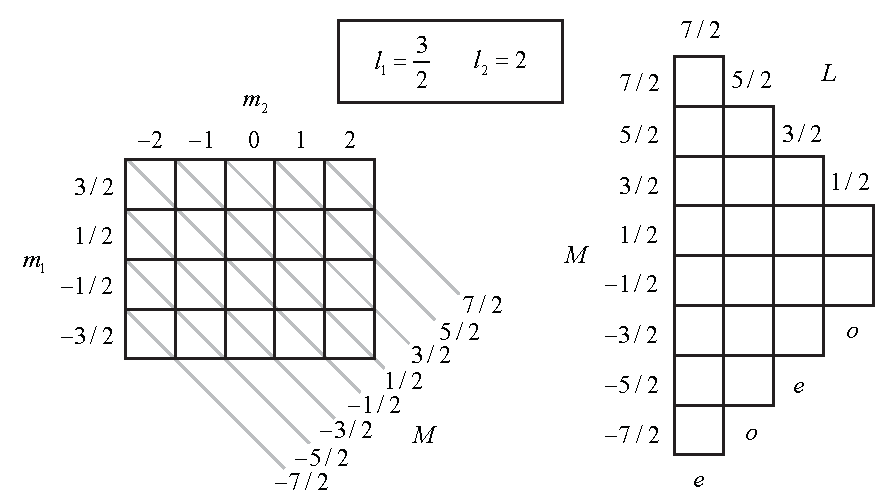
\includegraphics[width=14cm]{./figures/AMAdd_1.pdf}
\caption{图中每个方格代表一个基底. 这个空间也可以使用 $\ket{L, M}$ 作为基底, 且基底变换在每个 $M$ 子空间中独立进行} \label{AMAdd_fig1}
\end{figure}

\begin{equation}
N_M =
\begin{cases}
l_1 + l_2 - \abs{M} + 1 &(\abs{M} > \abs{l_1 - l_2}) \\
2\min\{l_1, l_2\}  + 1   &(\abs{M} \leqslant\abs{l_1 - l_2})
\end{cases}
\end{equation}
我们只需要在每个 $M$ 子空间中把 $L^2$ 算符对角化即可.
\begin{equation}
L^2 = L_1^2 + L_2^2 + 2(L_{1x} L_{2x} + L_{1y} L_{2y} + L_{1z} L_{2z})
\end{equation}
其中只有 $L_{1x} L_{2x} + L_{1y} L_{2y}$  不是对角矩阵.利用升降算符表示
\begin{equation}
2 (L_{1x} L_{2x} + L_{1y} L_{2y} ) = L_{1+} L_{2-} + L_{1-} L_{2+}
\end{equation}
\begin{equation}\ali{
&\quad \bra{l_1, m'_1, l_2, m'_2} L^2 \ket{l_1, m_1, l_2, m_2} = \hbar ^2 \times\\
& \qty[ \ali{
&\delta_{m'_1, m_1} \delta_{m'_2, m_2} [l_1(l_1 + 1) + l_2(l_2 + 1) + 2 m_1 m_2]  \\
+ &\delta_{m'_1, m_1 + 1} \delta_{m'_2, m_2 - 1} \sqrt{l_1 (l_1 + 1) - m_1(m_1 + 1)} \sqrt{l_2 (l_2 + 1) - m_2(m_2 - 1)}\\
+ &\delta_{m'_1, m_1 - 1} \delta_{m'_2, m_2 + 1} \sqrt{l_1 (l_1 + 1) - m_1(m_1 - 1)} \sqrt{l_2 (l_2 + 1) - m_2(m_2 + 1)} }]
}\end{equation}
 
矩阵的具体形式取决于基底的排列顺序. 把$\ket{L,M}$ 以 $L$ 从大到小的顺序排列, 基底 $\ket{l_1, m_1, l_2, m_2}$ ($m_2 = M - m_1$)以 $m_1$ 从大到小的顺序排列. 每组基底中 $m_1$ 的最大值为
\begin{equation}
\max \qty{m_1} =
\begin{cases}
l_1 \quad &(M \geqslant l_1 - l_2)  \\
l_2 + M &(M < l_1 - l_2)
\end{cases}
\end{equation}
这样, $L^2$ 的矩阵就是一个三对角矩阵,其本征矢矩阵就是从 $\ket{L, M}$ 表象到 $\ket{l_1, m_1, l_2, m_2}$ 表象的酉变换矩阵 $\mat U_M$.

查 CG 表时, CG 系数通常以 $\mat U_M$ 矩阵的形式给出(如 Griffiths).可以证明, $\mat U_M$ 的 $N_M$ 个本征值为 $L(L + 1) \hbar ^2$,  其中 $L = l_1 + l_2, l_1 + l_2 - 1,\dots$ (共 $N$ 项%未完成,不会证明
)(注意最小值大于但不一定等于 $\abs{M}$ ). $L$ 在所有子空间的最小值是 $\abs{l_1 - l_2}$ (当 $\abs{M} = \abs{l_1 - l_2}$ 时取得),所以 $L$ 在所有子空间的范围是
\begin{equation}
L = \abs{l_1 - l_2}, \dots, l_1 + l_2
\end{equation}
现在我们已经知道了每个子空间 $M$ 的变换,那么如何求总变换呢?先把总矩阵列表,行标题是所有的 $\ket{l_1, m_1} \ket{l_2, m_2}$, 列标题是所有的 $\ket{L, M}$, 对每个空间,找到对应的 $N$ 行和 $N$ 列,把 $N \times N$  的 $\mat U_M$ 矩阵照抄上去即可.

%未完成: 图中的 e 和 o 代表粒子交换的对称性, 推导一下为什么会是交替出现.
